\section{Related Work} % (fold)
\label{cha:related_work}
There has been a lot of research into image classification and object detection lately. A number of competitions have sparked development of a broad range of approaches to get the best results. There is not one correct way of performing object recognition, there is a multitude of methods that all have their merits and disadvantages. The NBNN approach also got more attention recently.

\subsection{Image Classification} % (fold)
\label{sec:image_classification}


\todo[inline]{Talk of related non-NBNN classification methods}
\JanTodo{codebook/BoW, Fisher kernel, Devil in the Details, BMVL, Chatfield}
% section image_classification (end)

\subsection{Object Detection} % (fold)
\label{sec:object_detection}

\todo[inline]{Talk of related non-NBNN detection methods (Get part based models and the like in here \ldots, and exemplar models )}

The most intuitive way of thinking about object detection is probably to apply image classification at various windows within the image instead of on the image as a whole. This involves iterating over possible window locations, sizes and aspect ratios for the whole image, and determining the likelihood of each window of representing an object. This so called sliding window approach marks early detection methods \cite{viola2004robust}. The applicability of this approach however is fairly limited, because of the large number of possible windows to check. Therefore, many methods find a way to make this window search more efficient. Viola \& Jones \cite{viola2004robust} propose a cascade approach, where a very simple classification method is used on the full set of hypotheses for bounding boxes in order to cast most of them away early. For difficult hypotheses a more sophisticated classification is done to narrow down the search, each step using a better, and much slower classification algorithm. In contrast, Efficient Sub-window Search methods \cite{behmo2010towards, lampert2008beyond, pedersoli2011coarse, yeh2009fast} model the problem into a branch-and-bound search method. They recursively split the window in two, find the response for the class on the current scale, and continue with the most promising leaf. When the response of both windows after a split is lower than the one above, the correct window is assumed to be on the above level.

Another approach that recently gained more attention because of the promising results it getting, is that of detection by segmentation. \cite{van2011segmentation,zhang2010free} These methods rely on the fact that segmentation methods are meant to subdivide the image into segments that represent a semantic unity, like parts of objects or full objects. The resulting segments can be used as hypotheses for detecting objects. This means the amount of possible windows can be reduced heavily. Van de Sande \emph{et al.} \cite{van2011segmentation} use a hierarchical segmentation algorithm to make the detection scale invariant, and train discriminatively by focusing on hard examples. Zhang \emph{et al.} \cite{zhang2010free} do not explicitly segment the image, but just like many segmentation algorithms they do look for edges that enclose an object as a restraint for selecting it as a possible detection.

Part-based models form a different approach on effectively finding hypothesis windows for objects \cite{felzenszwalb2010object}. These methods learn object models based on a combination and spatial organization of a number of designated, but unlabeled, parts. These parts are learned as a hidden variable during training, being groups of features reoccurring in the same formation in a certain area of bounding boxes of a class. Furthermore, the difference in scale between the full object window (the root) and its parts is fixed. In comparison with sliding-window approaches, this means a restriction in the number of possibilities for detection of objects. The relative scale of the parts should comply with that of the root scale.


\begin{figure}[hbt]
    \centering
    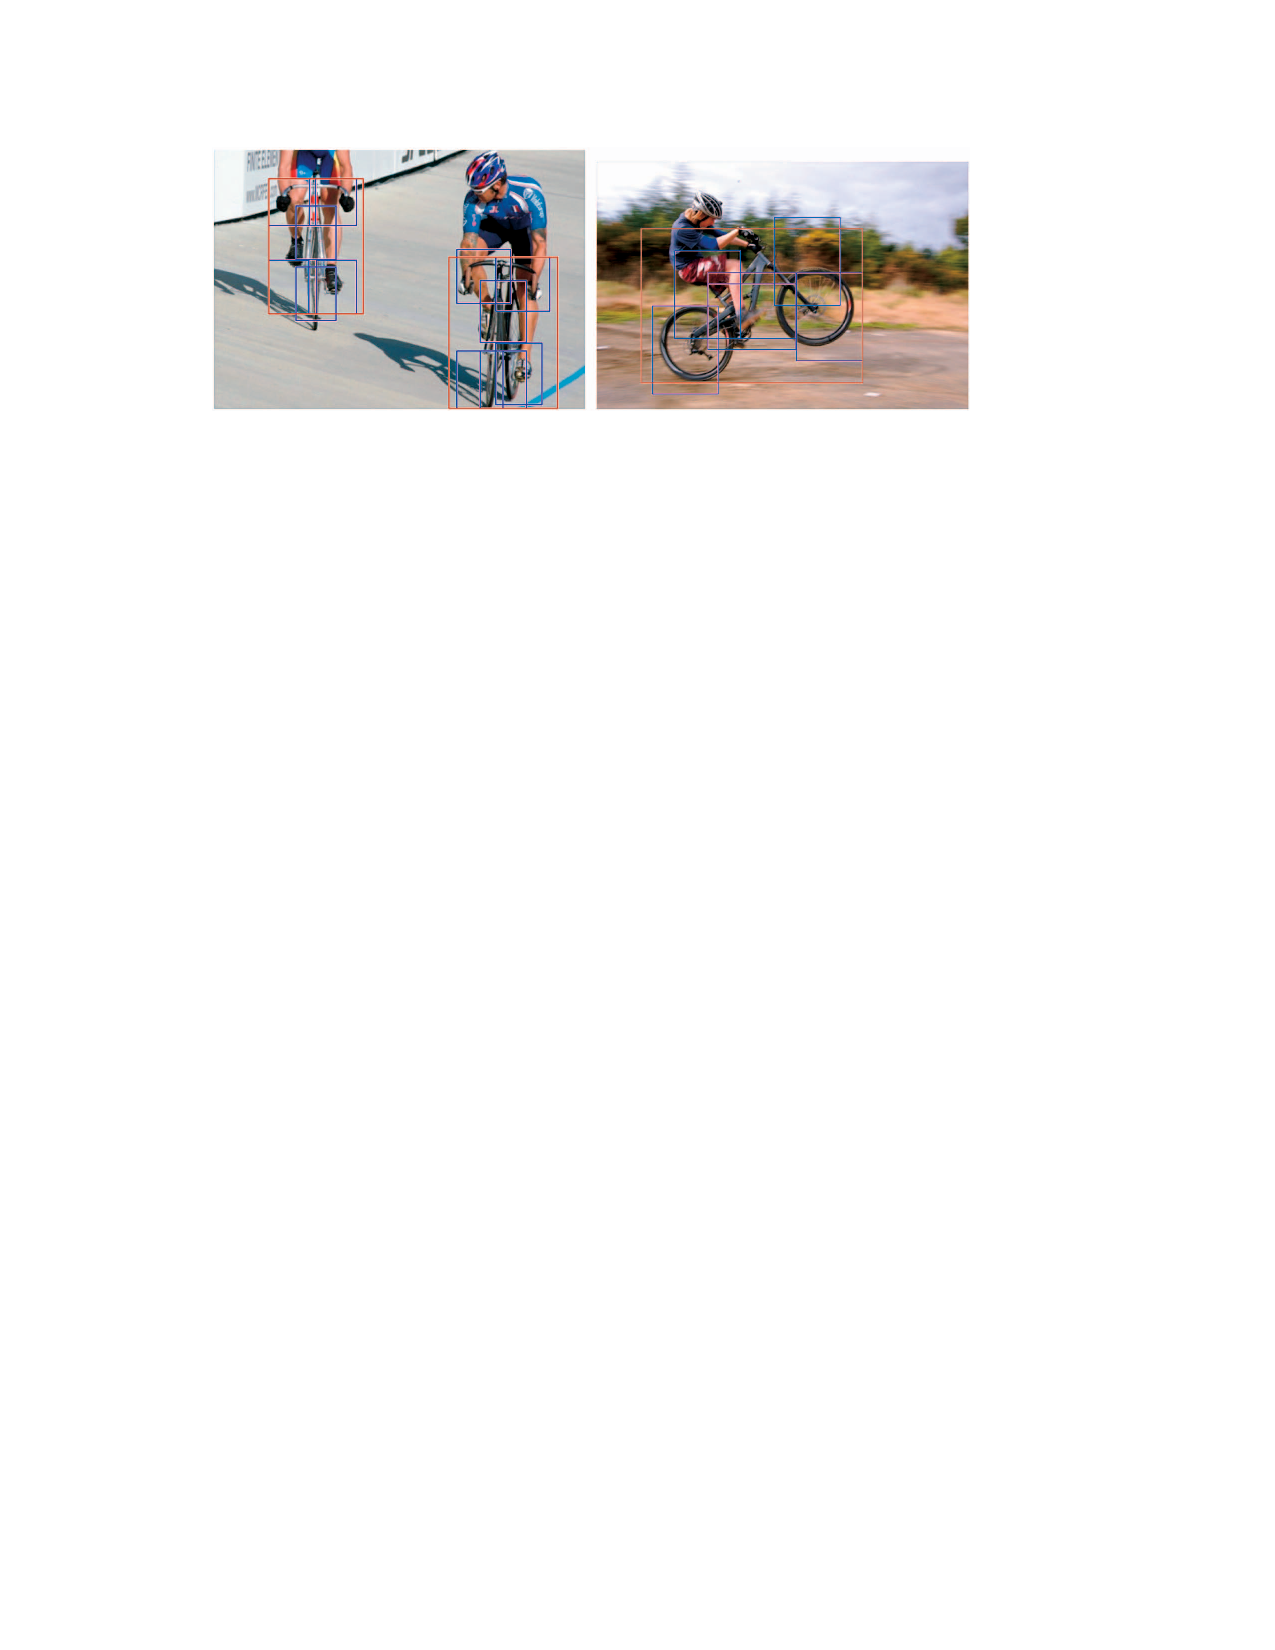
\includegraphics[width=0.8\textwidth]{PartBasedDet}
    \caption{From \cite{felzenszwalb2010object}.}
    \label{fig:partbaseddet}
\end{figure}

\begin{figure}[hbt]
    \centering
    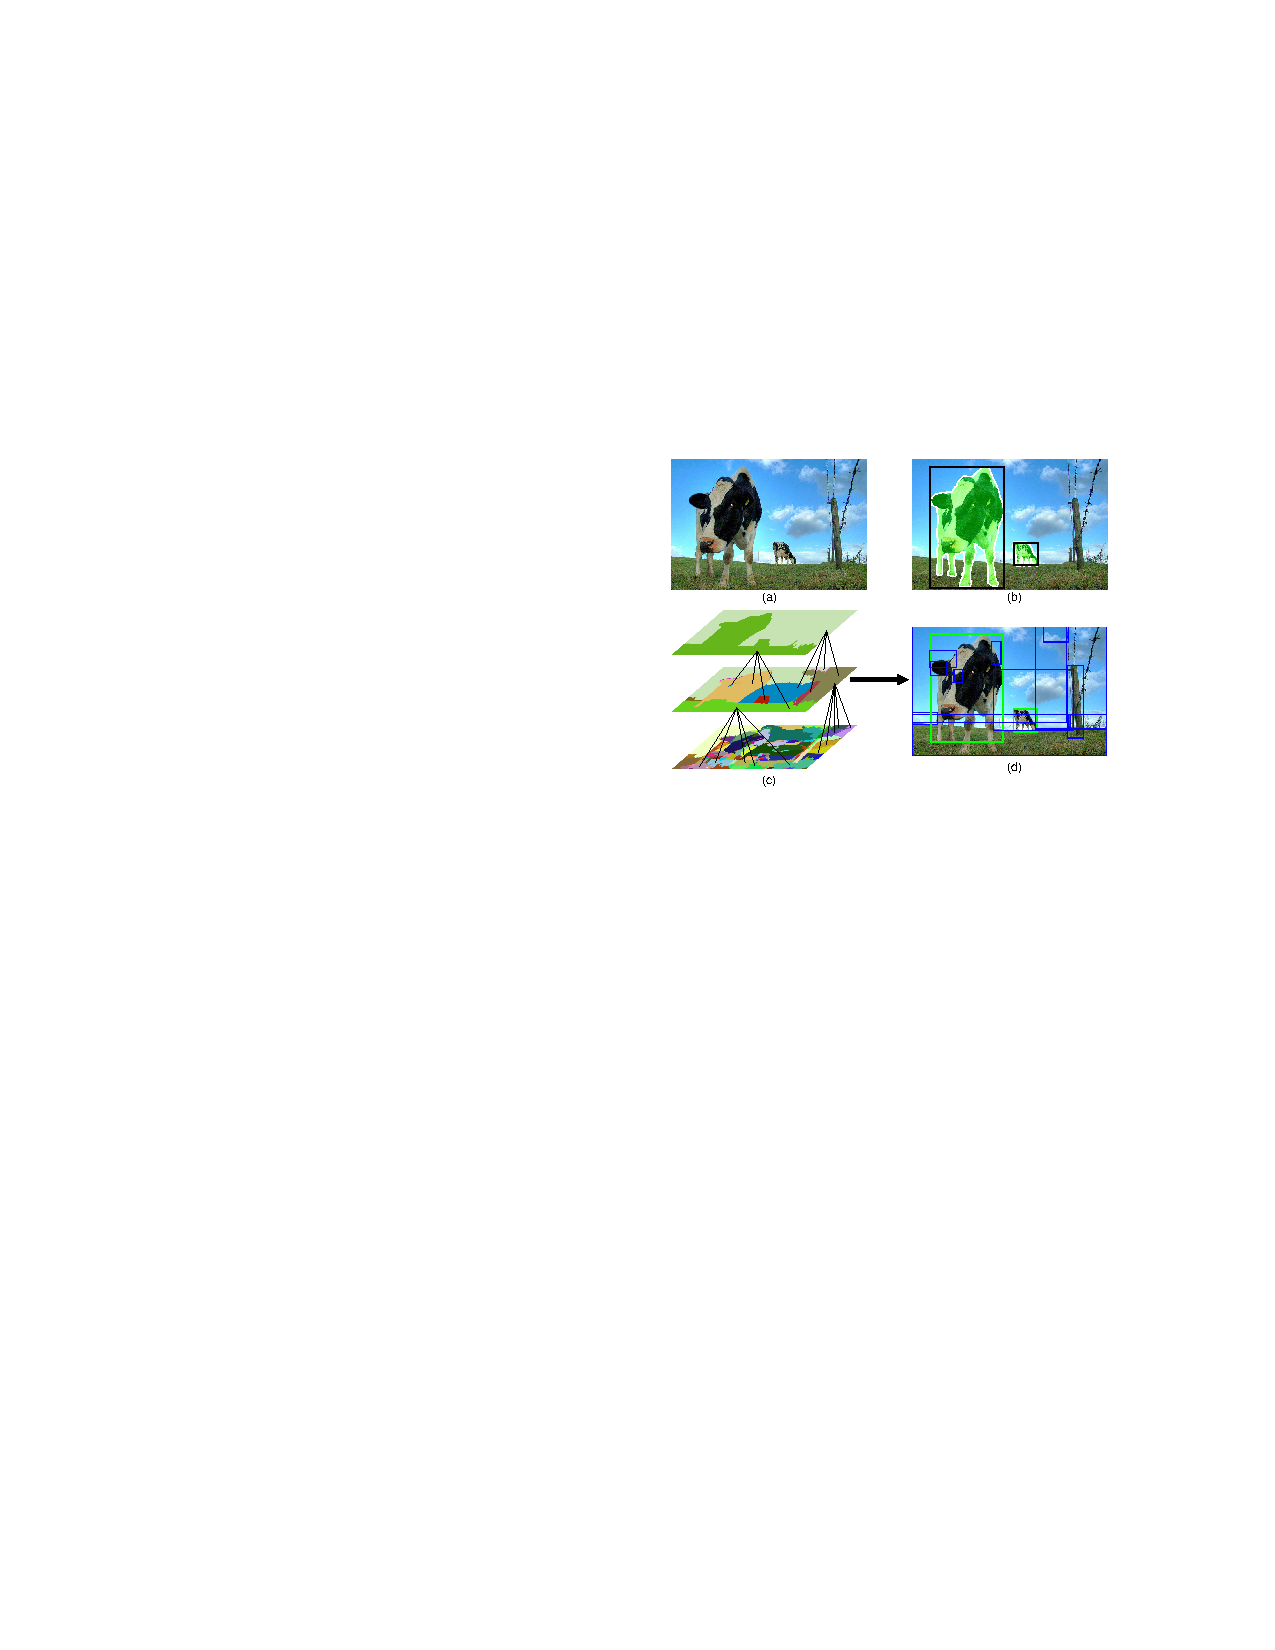
\includegraphics[width=0.8\textwidth]{LocByDet}
    \caption{``Given an image (a) our aim is to find its objects for which the ground truth is shown in (b). To achieve this, we adapt segmentation as a selective search strategy: We aim for high recall by generating locations at all scales and account for many different scene conditions by employing multiple invariant color spaces. Example object hypotheses are visualized in (d).'' From \cite{van2011segmentation}.}
    \label{fig:locbydet}
\end{figure}

% section image_detection (end)

\subsection{NBNN Based Methods} % (fold)
\label{sec:nbnn_based_methods}
\todo[inline]{Talk of Boiman shortly, and of methods related to it, up till the most recent ones, so include Tuytelaars, Becker, McCann, etc.\ldots}

Other limitations have been shown by various authors.\cite{behmo2010towards, mccann2012local,timofte2012iterative,tuytelaars2011nbnn,wang2011improved} Some authors \cite{behmo2010towards,wang2011improved} stress that NBNN is highly sensitive to differences in descriptor density over classes. Behmo \emph{et al.} for example state that this is caused by dropping the factor from the classification rule which normalizes for the descriptor density in the train set for a given class. This term is dropped because an equal kernel estimation is assumed, which does not hold for large differences in descriptor density over classes. \cite{behmo2010towards} Therefore, they propose to learn the density estimation parameters per class as a linear problem. This new formulation models an affine transformation on the distance measure used in NBNN. These two parameters can be seen as corrections for each class on the bias that arises when classes with the same priors are not equally sampled. Wang \emph{et al.} take a slightly different approach to solve the same problem. They try to correct the distances found by replacing the euclidean distance of NN by a learned Mahalonobis distance for each class 

% section nbnn_based_methods (end)